\chapter{直感的なリズムと旋律線の入力手法}
本章では身体動作で直感的にリズムと旋律線を入力する手法について述べる.

\section{RealSense SDK}
RealSenseを扱うためのRealSense SDKが提供する機能のうち,本研究で使用したものを述べる.
\subsection{RealSenseのジェスチャー認識}
RealSense SDKでは,図\ref{img:jesture}に示す11種類のジェスチャーが定義されている.しかし,あらかじめ定義されているジェスチャーの多くは,認識精度に問題があり,認識漏れや遅延が発生する.音楽を演奏するインタフェースの操作手段としてジェスチャーを使用するにはこの遅延が大きな障害となる.本研究ではジェスチャー認識に加えて,手指や手のひらの座標,開閉度などのパラメータを利用して認識精度を向上させた.
\begin{figure}[t]
	\begin{center}
		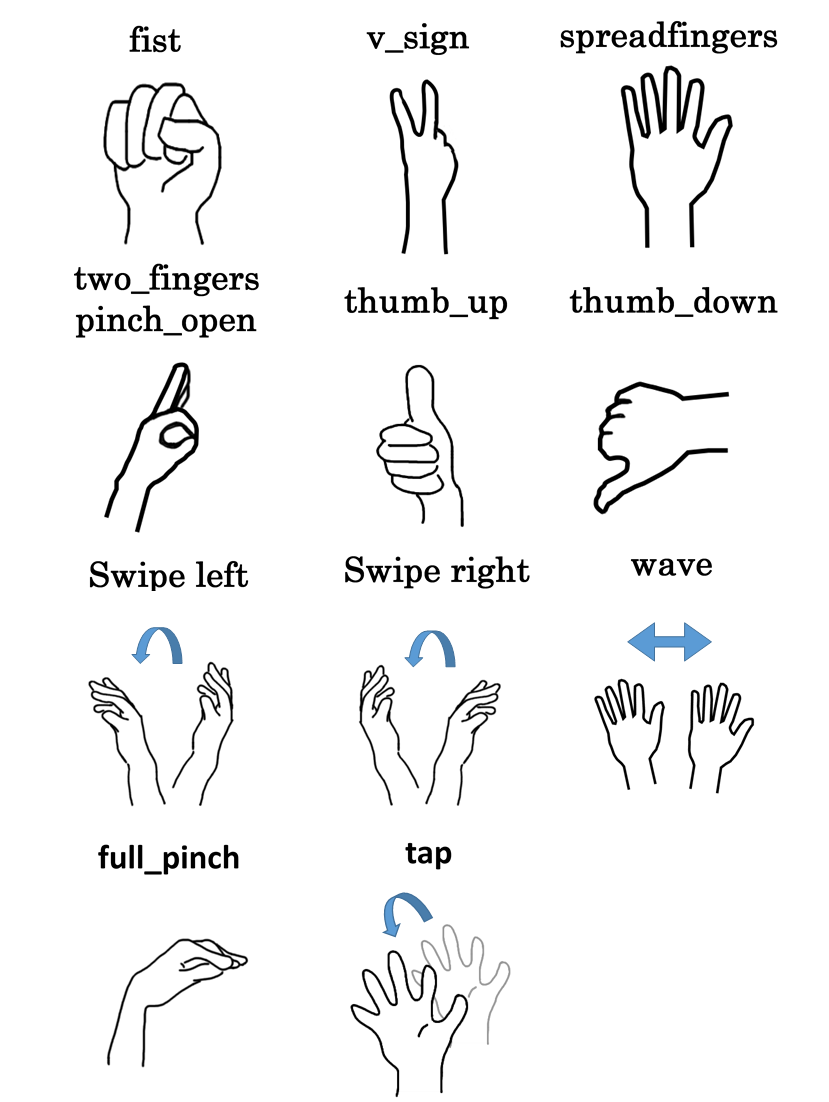
\includegraphics[width=0.9\linewidth]{assets/img/jesture.png}
		\caption{11種類のジェスチャー}
		\label{img:jesture}
	\end{center}
\end{figure}

\subsection{関節の認識}
RealSenseカメラでは図\ref{img:handlabels}に示す22種類の手のひらの関節を認識することができる.本研究では図\ref{img:handlabels}のMiddle Fingertipの座標を指先の座標,Palmの座標を手のひらの座標として扱った.
\begin{figure}[t]
	\begin{center}
		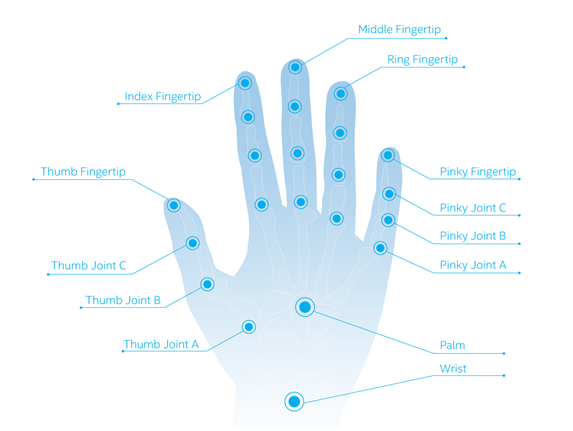
\includegraphics[width=1\linewidth]{assets/img/hand_labels.png}
		\caption{22種類の関節\cite{hand_labels}}
		\label{img:handlabels}
	\end{center}
\end{figure}

\section{持続音と減衰音}
持続音とはバイオリン,笛などのような音量が一定のまま鳴り続ける音で,減衰音とはピアノ,鉄琴,木琴などのような音量が減衰していく音である.
本研究ではユーザの演奏表現にバリエーションを提供するために持続音と減衰音の両方を扱う.よってユーザーが好きな時に持続音と減衰音を切り替えられるように,図\ref{img:jesture}のうちthumb\_up動作をすると演奏音が持続音か減衰音に切り替わるように割り当てた.
本研究では左右の手で出力される演奏音は独立しており,2和音まで出力可能である.

\subsection{旋律線の入力}
図\ref{img:note1}に身体動作による旋律線の入力の概要を示す.ジェスチャーで音の種類を持続音に指定しユーザーはRealSenseの前で動くと指先の座標の時間的変化がそのまま旋律線として入力される.Processing側では画面を現在発音可能な演奏音の数で等分割した領域を用意して,インタフェースの画面に色分けして表示する.手指の座標がどの領域に存在するかにより,その領域とひも付けられた背景楽曲の調性制約を満たす周波数の音が演奏音として出力される.
\begin{figure}[t]
	\begin{center}
		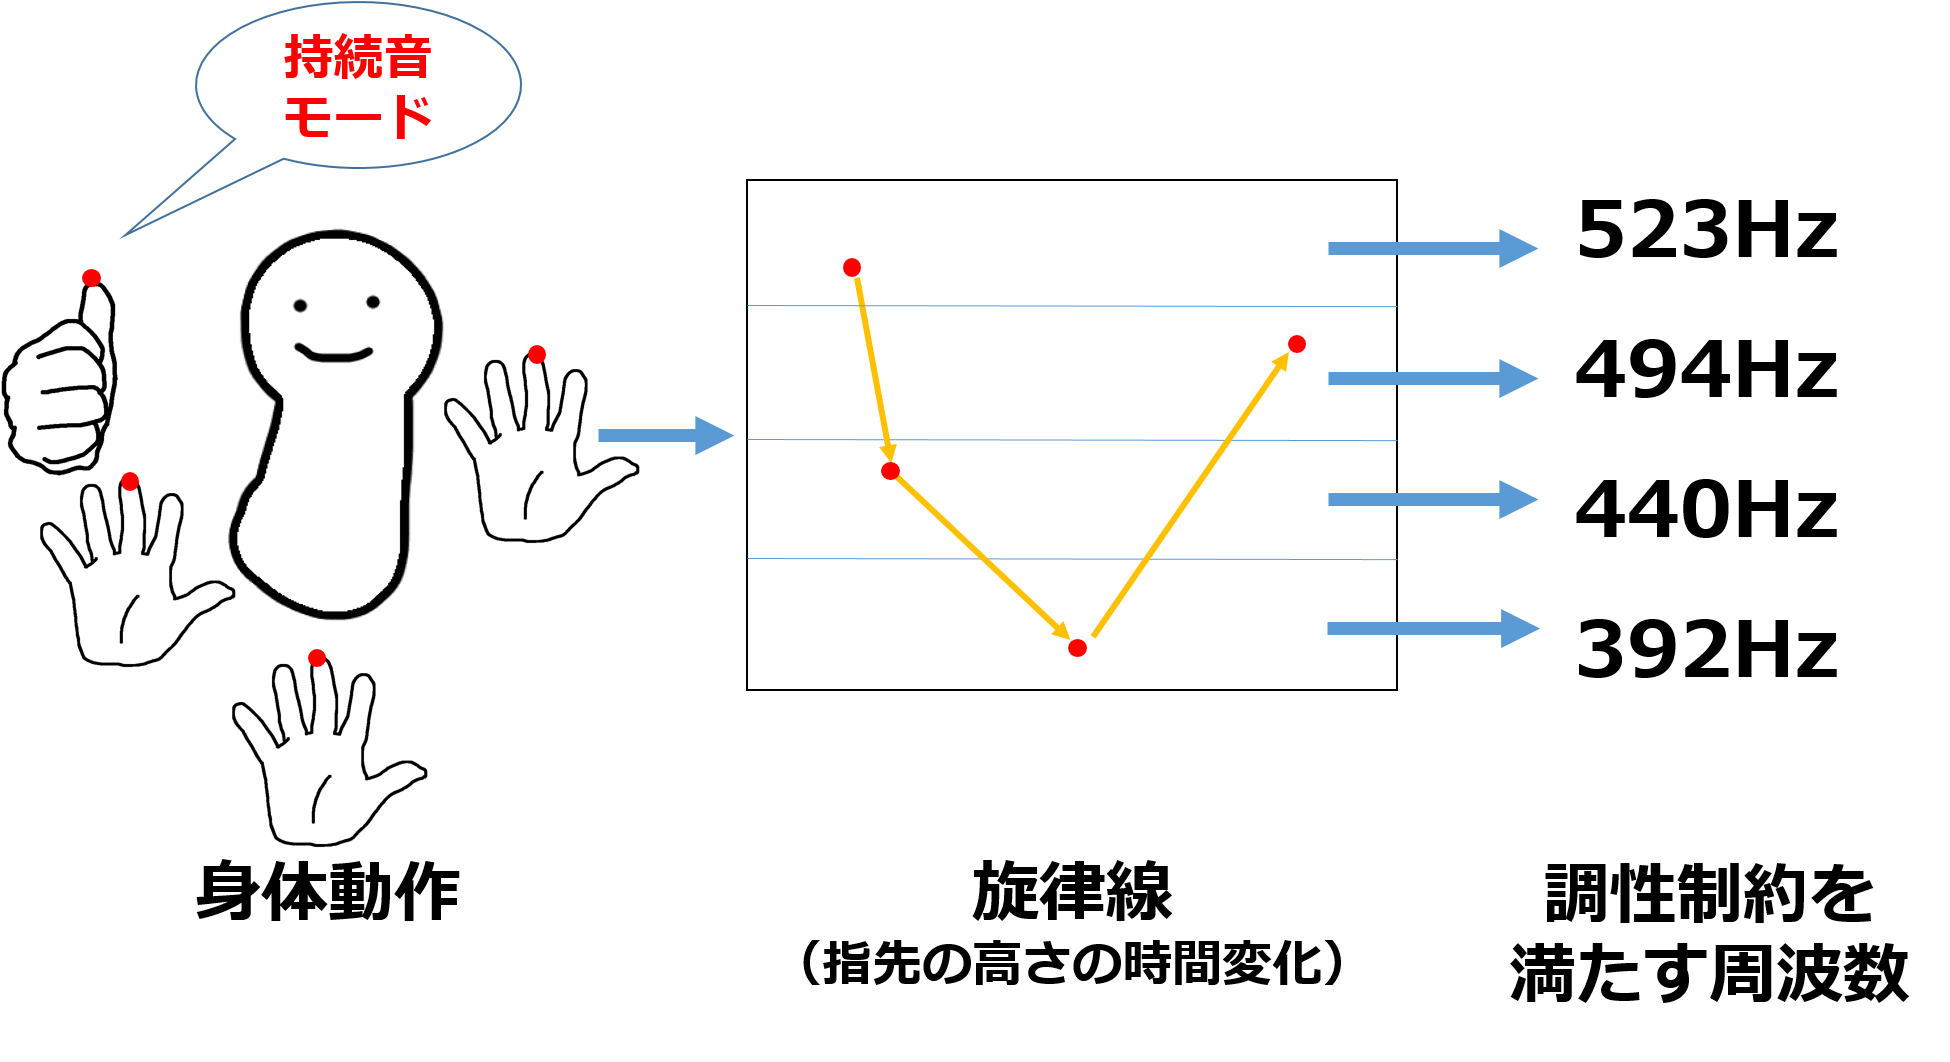
\includegraphics[width=0.9\linewidth]{assets/img/in_note.png}
		\caption{直感的な旋律線の入力方法}
		\label{img:note1}
	\end{center}
\end{figure}
\subsection{リズムの入力}
持続音を出力する際に現在演奏している音の領域と離れた領域の音を出力する場合,手を移動させた時に通った領域の音まで出力してしまう.そこでSongle Web APIから取得した背景楽曲の拍に合わせて点滅する円を画面に表示させ,リズムを取りやすくするとともに,円が表示されてないタイミングのとき演奏音をportamentoを設定することで,離れた領域の音を出力するときに間の領域の音を出力するのを防ぐ.本研究では点滅する円に合わせるようにして手を動かすことをリズムの入力とした.図\ref{img:portamento}に拍とportamentoのタイミングを示す.曲のビート一拍分を半分に分けた時の前半部分の間に円を表示させ,後半部分の間に円を非表示にしてportamentoを設定する.後半部分の間指先を動かして領域を移動すると,出力音は滑らかに変化する.
\begin{figure}[t]
	\begin{center}
		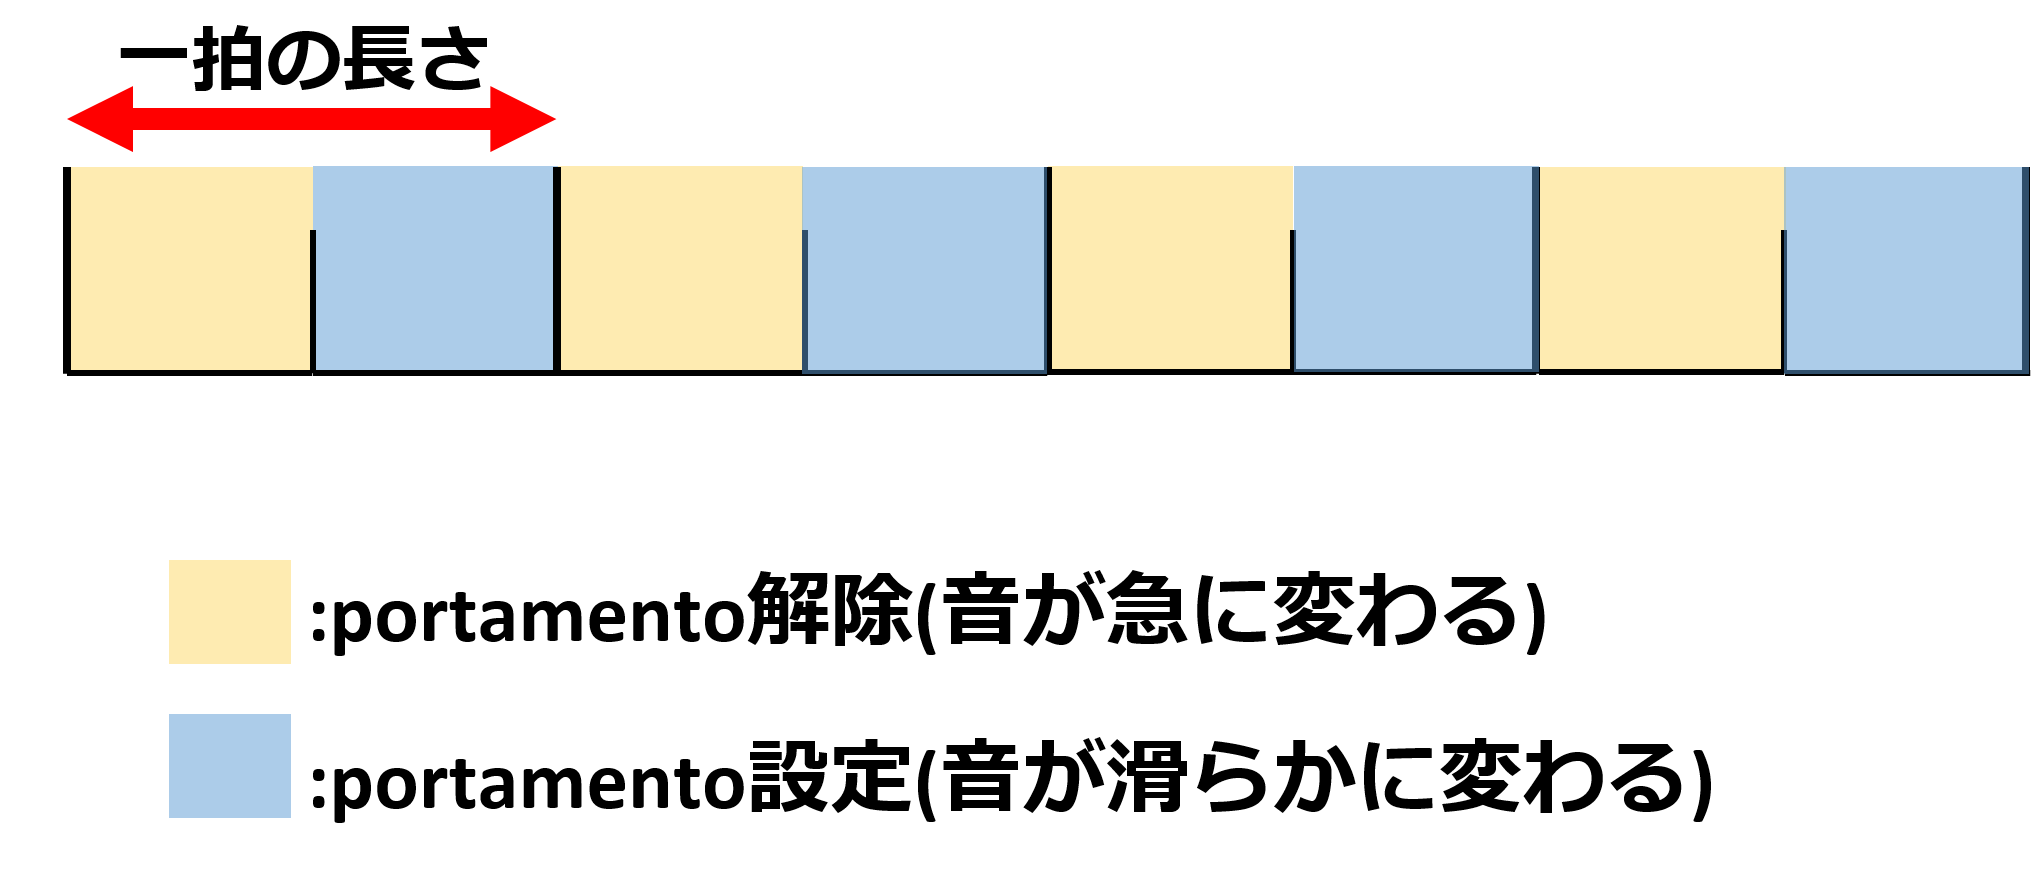
\includegraphics[width=1\linewidth]{assets/img/portamento.png}
		\caption{拍とportamentoのタイミング}
		\label{img:portamento}
	\end{center}
\end{figure}
\subsection{持続音のジェスチャー}
持続音のオンセットとオフセットには,それぞれ図\ref{img:jesture}のspreadfingersとfistを割り当てた.これらのジェスチャーの精度を向上させるため,指の開閉度というパラメータ(0〜100)を利用した.ジェスチャー認識の条件に開閉度が90以上の時,spreadfingers動作を,1fあたりの変化量が-10を下回った時,fist動作をするように設定させた.
\subsection{減衰音のジェスチャー}
減衰音のオンセットには図\ref{img:jesture}のtap動作を割り当てた.本研究の持続音は1秒間だけ出力されるので減衰音のオフセットにジェスチャーは割り当ててない.tap動作をしたとき指先の座標が存在する領域に対応した周波数の音が出力される.tap認識の精度を向上させるため,指先と手のひらの速さと移動距離に閾値を設定したときtap動作をしたと認識させた.図\ref{img:tap}に閾値を設定した場所を示す.閾値は経験的に指先のz座標のカメラ方向への移動距離が20mm以上移動した時,指先の3次元移動速度が1.8m/s以上,手のひらの移動速度が0.6m/s以上1.5m/s以下の時tap動作とした.本研究のtap動作はRealSense SDKのtap認識の代わりに使用しているため,どちらが優れているかの評価実験を行い,第6章でまとめた.
\begin{figure}[t]
	\begin{center}
		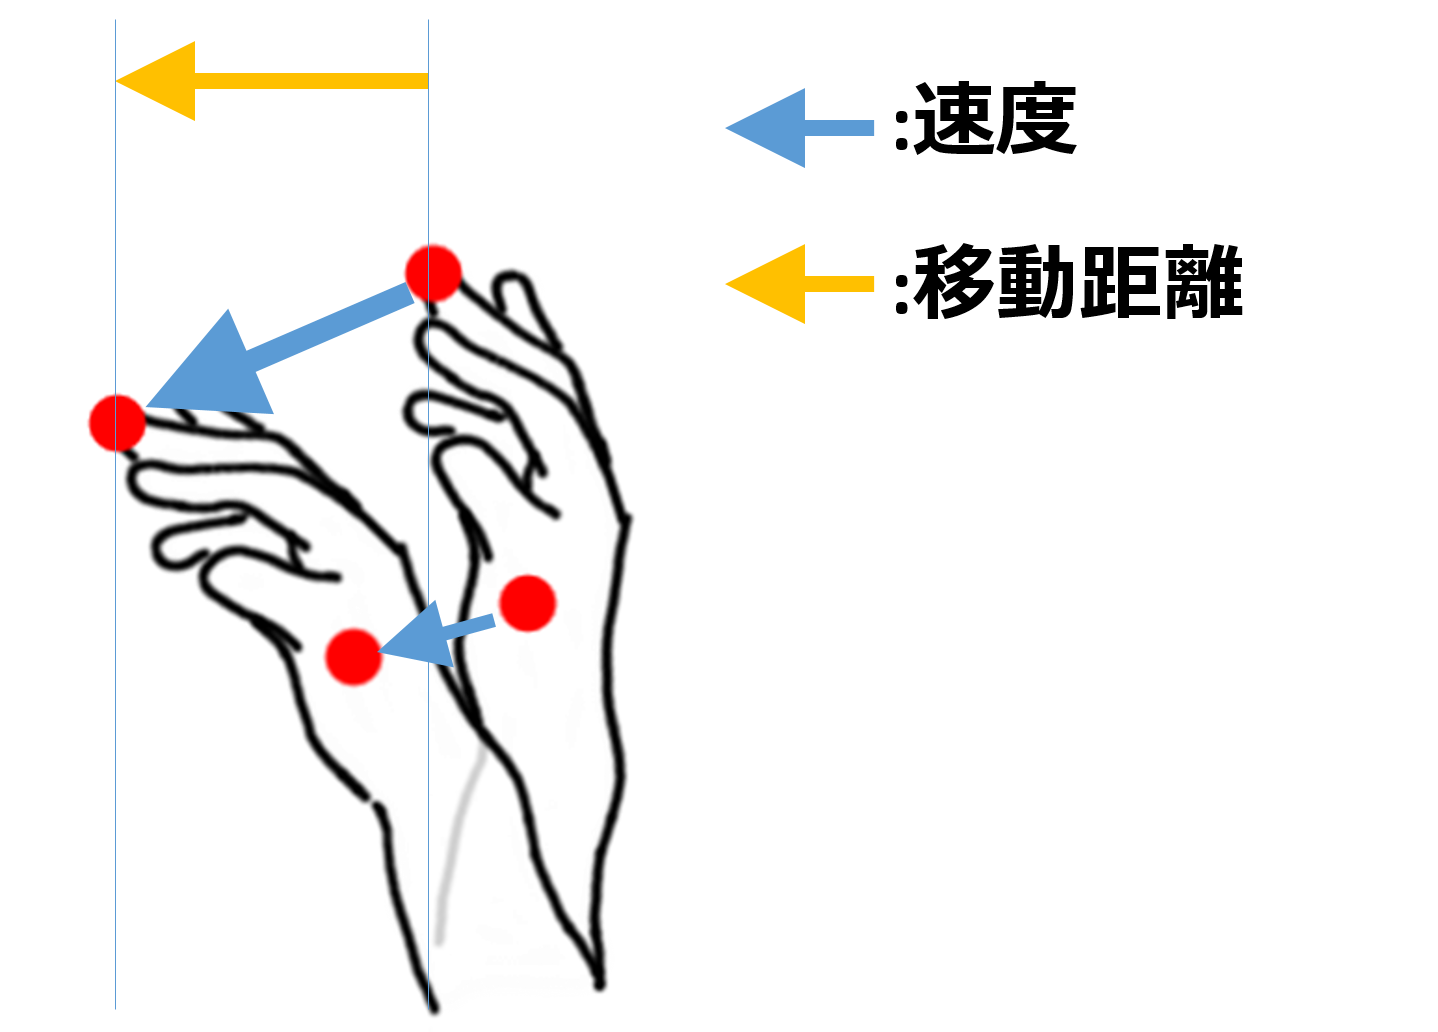
\includegraphics[width=1\linewidth]{assets/img/tap.png}
		\caption{tap動作の閾値}
		\label{img:tap}
	\end{center}
\end{figure}
\subsection{実行結果}
図\ref{img:interface_result1},図\ref{img:interface_result3}に実行結果を示す.画面下の拍によって点滅する円である.指先の小さい円が指先の座標を表し,領域の色が濃くなっているところが現在指定している高さの領域である.赤になるほど音が高く,緑になるほど音が低くなる.
\begin{figure}[t]
	\begin{center}
		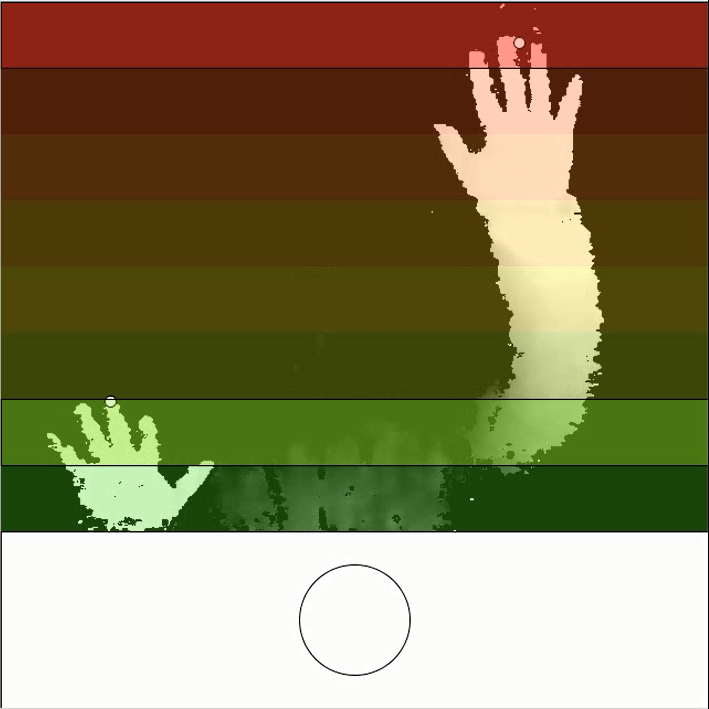
\includegraphics[width=0.5\linewidth]{assets/img/result1.png}
		\caption{実行結果1}
		\label{img:interface_result1}
	\end{center}
\end{figure}
\begin{figure}[t]
	\begin{center}
		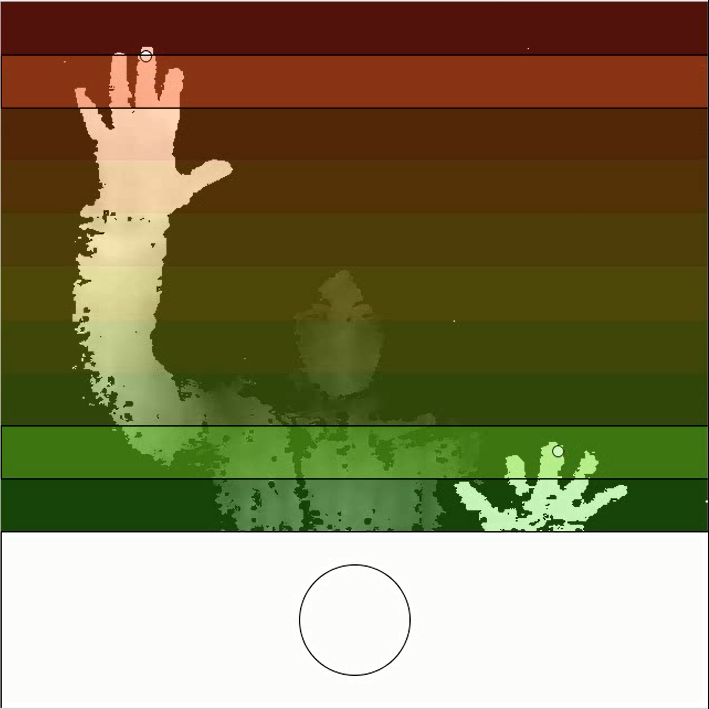
\includegraphics[width=0.5\linewidth]{assets/img/result3.png}
		\caption{実行結果2}
		\label{img:interface_result3}
	\end{center}
\end{figure}
